
\chapter{基于术语识别边界信息的术语识别和翻译方法}
\label{Chapter_term}

术语(terminology)是在特定学科领域用来表示概念的称谓的集合,在本文中主要指专业领域中的科技名词,即科技术语,如“数据库(database)”、“进程间通信(IPC)”等。在微软本地化翻译语料中,平均每100个词就包含15个术语。由于缺乏专业背景知识,专业译员花费大量时间来查证术语翻译。同时,每天都在产生新的科技术语。

可见,术语翻译对于专业领域的人机交互式机器翻译至关重要且充满挑战,本章将探讨如何改善专业领域的术语翻译质量。术语翻译知识来源多样,维基百科、普通网页和双语平行句对中都可能有大量的术语翻译知识。所以,如何将已有的术语翻译知识挖掘出来并有效地融合进机器翻译中尤为重要。

现有机器翻译系统往往没专门考虑术语的翻译问题,主要表现在下列三个方面:(1)我们没有充分利用机器翻译训练语料中的术语翻译知识。在训练语料的双语平行句对中就有大量的术语翻译对,但在传统的训练流程中,一般只将这些术语当作普通词对待。因此在词对齐和翻译规则抽取中,这种区分术语词和非术语的处理方式引入了大量噪声。(2)互联网上的术语翻译知识也没有得到有效挖掘和利用。维基百科和普通网页中带双语括号的句子就包含大量的双语术语对。(3)现有融合术语翻译知识的方式较为单一。一般是先将挖掘到的双语术语作为术语翻译表引入机器翻译系统,机器翻译解码器在翻译过程中通过直接查表的方式将术语翻译结果插入目标译文。如果源语言术语识别或者匹配错误,则术语翻译错误直接影响整句翻译质量。

因此,我们提出了基于术语识别边界信息的术语识别和翻译方法。由于当前术语识别的性能还比较低,我们根据术语识别边界信息建立滑动窗口以动态扩展或收缩术语,借助术语识别边界信息建立术语解码方法,充分利用从平行句对和互联网单语语料中挖掘得到的术语翻译知识。该方法包括三个部分:从平行句对中挖掘术语翻译知识的融合双语术语识别的联合词对齐模型,从单语语料中挖掘术语翻译知识的基于双语括号句子的术语翻译挖掘方法,以及基于术语识别边界信息的统计翻译术语解码方法。

本章的组织结构如下: 4.1节和4.2节分绍讨论如何从双语平行句对和互联网单语语料中挖掘出带上下文信息的术语翻译知识,即融合双语术语识别的联合词对齐方法和基于双语括号句子的术语翻译挖掘方法;然后在4.3节中介绍融合术语识别边界信息的统计翻译术语解码方法;4.4节给出实验和分析,最后的4.5节对本章进行总结。

\section{融合双语术语识别的联合词对齐方法}

\begin{figure}[!tb]
	\centering
	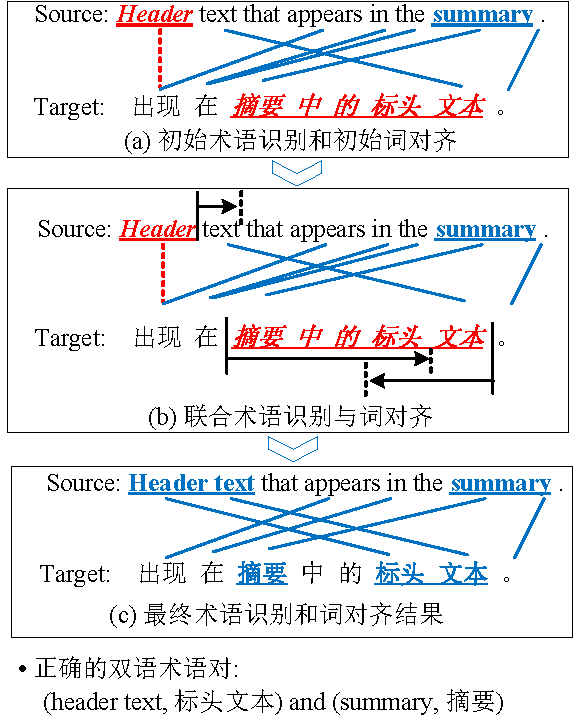
\includegraphics[width=0.6\textwidth]{Figure/Figure_4_1.pdf}
	\caption{融合双语术语识别的联合词对齐方法概览。红色表示错误的结果,蓝色表示正确的结果。}
	\label{Fig_joint_term_overview}
\end{figure}

词对齐是统计机器翻译的一项核心任务,它从双语平行语料中发掘互为翻译的语言片断,是翻译知识的主要来源。在实践中,一部分词对齐错误就是术语产生的,最终的译文质量也会受到影响。如果能自动识别出平行句对中的术语对应关系,词对齐质量就能得到改善,进而有望改善术语和句子的翻译质量。

术语识别方面,基于规则的方法已基本退出历史舞台。基于统计方法的方法虽然不受领域限制,但是对于多词术语和低频术语的识别并不理想,因而抽取的术语也存在较多噪声。其主要原因为如下两点:(1)性能更好的基于机器学习的术语识别方法需要高质量的人工标注数据,但目前极度缺乏大规模高质量的术语标注数据;(2) 不断有新的术语产生,标注数据的更新速度严重滞后于实际需求。所以,如果直接将术语识别结果作为词对齐的约束,术语识别错误就会传递给后续阶段,最终译文质量反而难以得到提升。因此,研究如何提高术语识别和词对齐性能,并提高最终的机器翻译译文质量是迫切需要解决的一个难题。

在本章中,为了尽量降低训练流程中错误传递的影响以改进术语翻译知识抽取,我们提出了融合双语术语识别的联合词对齐方法。首先,为了降低对训练数据的依赖,该联合词对齐方法从单语术语识别弱分类器开始。该分类器由维基百科等自然标注数据训练得到的。其次,为了降低因术语识别和词对齐的错误传递带来的负面影响,该方法利用双语术语和词对齐的相互约束,将单语术语识别、双语术语对齐和词对齐联合在一起执行,最后得到效果更好的双语术语识别和词对齐结果。该联合词对齐方法的步骤如图\ref{Fig_joint_term_overview}所示。

图4.1的起点是性能较弱的基于最大熵的英文和中文单语术语识别分类器,以及基于隐马尔可夫模型的词对齐模型。在图\ref{Fig_joint_term_overview}(a)中,有3处比较明显的错误:(1)英文词“header”被错误地对齐到了“出现”;(2)第一个英文术语“header text”被错误地识别成了“header”;(3)“摘要中的标头文本”很显然不是一个术语,而应该被识别为两个术语,即“摘要”和“标头文本”。另外,识别出的术语也没有被正确对齐,而且非术语词与术语中的词相互交错。因此,这样的词对齐和术语识别结果是不能用来抽取翻译知识的。

幸运地是,经过对图\ref{Fig_joint_term_overview}(a)中的示例分析,我们有三个比较重要的发现:(1)初始识别结果虽然不一定完全正确,但可以作为进一步识别的锚点。比如我们可以扩展“header”的右边界,使“header text”能被正确识别。(2)在平行句对中,双语术语一般都是成对出现的。因而,词对齐结果应该有利于单语术语边界的确定。例如“summary”被识别为源端术语,那么与它对齐的“摘要”也应该是目标端术语。(3)双语术语的对齐约束也同样有利于词对齐的确定。如果“header text”与“标头文本”被识别为术语翻译对,那么这两个术语内的词就不应该与其它词对齐,因而“header”被错误对齐到“出现”这种错误可以被纠正。由此可以发现,同时识别双语术语与词对齐能够突破分别单独进行双语术语识别和词对齐的局限性,从而有望大幅提高双语术语识别与词对齐的性能。

基于上述分析,我们提出的联合词对齐方法,如图\ref{Fig_joint_term_overview}(a)将单语术语识别结果作为锚点,然后如图\ref{Fig_joint_term_overview}(b)建立滑动窗口以动态扩展或收缩术语,最后得到如图\ref{Fig_joint_term_overview}(c)的词对齐和双语术语识别结果。我们将上述过程形式化为四阶段联合词对齐模型,接下来,我们将详细讨论该模型以及一些重要推导细节。

\subsection{词对齐的四个阶段}

\begin{figure}[!tb]
	\centering
	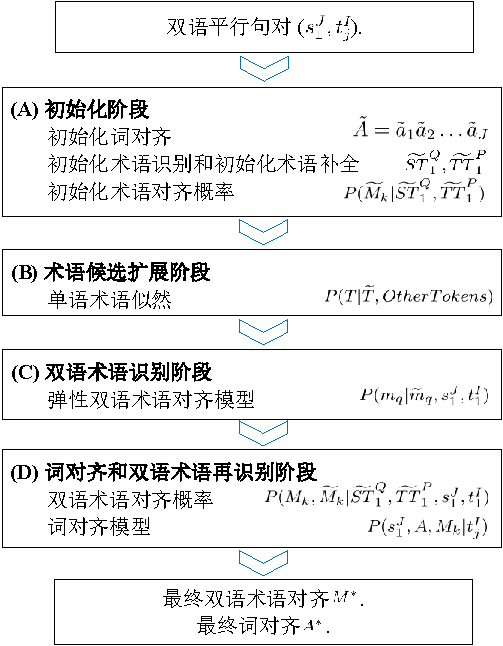
\includegraphics[width=0.6\textwidth]{Figure/Figure_4_2.pdf}
	\caption{四阶段联合词对齐模型}
	\label{Fig_joint_term_model}
\end{figure}

在本章中,我们用四阶段联合词对齐模型将双语术语识别和词对齐两项任务融合在一起执行,同时允许词对齐与单/双语术语识别进行交互,最后改善术语和句子翻译知识的抽取。如图\ref{Fig_joint_term_model}所示,词对齐的整个过程可以分为四个阶段:

(A)\textbf{初始化阶段},利用自然标注数据训练的单语术语识别弱分类器得到初始源语言术语和初始目标语言术语,即初始化术语对齐。

(B)\textbf{术语候选扩展阶段},将初始术语对齐作为锚点建立滑动窗口以动态扩展或收缩术语,计算单语术语似然,获得扩展双语术语候选列表。

(C)\textbf{双语术语识别阶段},利用弹性双语术语对齐模型,结合扩展双语术语候选列表,进行双语术语识别,得到修正后的双语术语候选列表。

(D)\textbf{词对齐和双语术语再识别阶段},同时进行第二次双语术语识别和词对齐,得到最终的双语术语识别和词对齐结果。

\textbf{(A)第一阶段:初始化阶段}

令源语言句子为$ s_1^J=s_1s_2\ldots s_J$,目标语言句子为$ t_1^I=t_1 t_2\ldots t_I$,其中$J$和$I$分别为源语言句子和目标语言句子的词的数目。第一阶段的起点是自然标注数据训练的单语术语识别弱分类器。初始化阶段一共有四个步骤:初始化词对齐、初始化术语识别、初始化术语补全和初初始化术语对齐。

初始化词对齐:在本章中,我们采用基于隐马尔可夫模型(HMM)的词对齐[\cite{Vogel:1996}]模型。给定源语言-目标语言句子对$(s_1^J,t_j^I)$,我们可以由预先训练好的HMM词对齐模型得到初始化词对齐结果$\tilde{a}_j=\{i|a(j)=i\}$。其中,$t_i$表示目标语言句子中的词 对应源语言句子中的词$j_i$。预先训练HMM词对齐模型的语料为数百万同领域双语平行句对。

初始化术语识别:给定双语句对$(s_1^J,t_j^I)$,由预先训练好的单语术语识别器得到初始化源语言术语集合$\widetilde{ST}_1^Q$和目标语言术语集合$\widetilde{TT}_1^P$,其中,$Q$和$P$分别表示源语言和目标语言术语的个数。预先训练的单语术语识别分类器基于开源的Stanford Classifier[\cite{Manning:2003}],其结果类似于“Header/B text/I that/N appears/N in/N the/ summary/U ./N”。每个词的标签可能为“U”(单词术语,即只包含一个词的术语)、“B”(术语起始词,即术语的第一个词)、“I”(术语词,即术语中第二个及以后的词)或者“N”(非术语词)。我们使用基于柱搜索算法的术语识别解码器将分类器结果的标签序列解码为合法的术语识别结果,例如:标签“U”必须在标签“N”之后,标签“B”之后必为标签“I”。

初始化术语识别结果仅作为后续阶段扩展或者收缩的锚点,则初始化术语识别的召回率越高越好。维基百科在内的自然标注数据训练的单语术语识别分类器就有比较高的召回率。所谓自然标注指人们在句子中插入的超链接、粗体、斜体或引号等格式标记。另外,为了将自然标注的数据转换为初始化术语识别分类器的训练语料,除了需要一定的人工清理成本,还需要将这些标注信息转换成如图\ref{Fig_joint_training_example}所示的标签序列。

初始化术语补全:源语言术语和目标语言术语成对出现在双语平行句对中。为了降低遗漏,初始化源语言术语集合$\widetilde{ST}_1^Q$和初始化目标语言术语集合$\widetilde{TT}_1^P$需要按照如下规则进行补全:如果源语言术语$\widetilde{ST}_q$中所有词对应的目标语言词都没有被识别为术语词,那么将这些目标语言词中最有可能为术语的作为单词术语添加到$\widetilde{TT}_1^P$;针对所有初始化目标语言术语进行类似操作。

\begin{figure}[!tb]
	\centering
	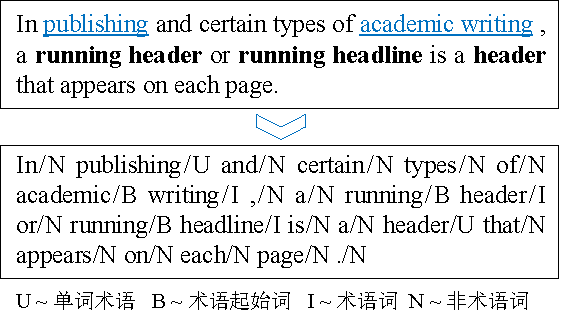
\includegraphics[width=0.6\textwidth]{Figure/Figure_4_3.pdf}
	\caption{将自然标注句子转换为初始化术语识别分类器训练语料的示例。蓝色下划线表示超链接。}
	\label{Fig_joint_training_example}
\end{figure}

初始化术语对齐:通过源语言术语集合$\widetilde{ST}_1^Q$和目标语言术语集合$\widetilde{TT}_1^P$的笛卡尔集生成初始化术语对齐集合$\widetilde{M}=\widetilde{M}_1^{(P^Q)}$。在术语对齐过程中,用预先训练好的术语对齐模型对集合$\widetilde{M}$中的所有元素进行打分并按降序排列。第$k$个可能的对齐为$\widetilde{M}_k=\widetilde{m}_1\widetilde{m}_2\ldots\widetilde{m}_Q  $,其中$\widetilde{m}_q=(\widetilde{ST}_q, \widetilde{TT}_p)$,$1 \le p \le P$并且$1 \le q \le Q$。

在本章中,预先训练好的术语对齐模型是基于最大熵模型实现的。训练语料包括维基百科双语标题和领域相关的双语术语表。特征包括双向短语翻译概率、双语词汇化翻译概率和共现频率。其中,由基于隐马尔可夫的词对齐模型计算词汇化翻译概率。这里的词对齐模型的训练语料是维基百科的双语标题和领域相关的双语术语表,不同于初始化词对齐模型所采用的双语平行句对。

对于图\ref{Fig_joint_term_overview}中的示例而言,第一阶段的输入包括下列项:

\begin{center}
	\begin{boxedminipage}[h]{\linewidth}
		\small
		\quad (1)初始化词对齐:
		
		 \qquad\qquad\qquad ``NULL\{3\} 出现\{1,4\} 在\{5,6\} 摘要\{7\} 中\{\} 的\{\} 标头\{\} 文本\{2\} 。\{8\}''
		
		\quad(2)初始化术语识别 
		
		\qquad \qquad $\bullet$ 带术语标记的英文(源语言)句子:
		
		\qquad\qquad\qquad ``\textless Header\textgreater \space text that appears in the \textless summary\textgreater \space.'' 
		
		\qquad \qquad $\bullet$ 带术语标记的中文(目标语言)句子:
		
		\qquad\qquad\qquad ``出现 \  在 \ \textless摘要 \ 中 \ 的 \ 标头 \ 文本\textgreater \ 。''
		
		\quad (3)初始化术语识别结果:
		
		\qquad \qquad $\bullet$ 初始化英文(源语言)术语识别结果:
		
		\qquad\qquad\qquad ([header], [summary])
		
		\qquad \qquad $\bullet$ 初始化中文(目标语言)术语识别结果:
		
		\qquad\qquad\qquad ([摘要\ 中\ 的\ 标头\ 文本])
	\end{boxedminipage}
\end{center}

输出则包括下列项:

\begin{center}
	\begin{boxedminipage}[h]{\linewidth}
		\small
		\quad (1)补全后的初始化术语
		
		\qquad \qquad $\bullet$ 补全后的初始化英文(源语言)术语识别结果:
		
		\qquad\qquad\qquad ([header], [summary])
		
		\qquad \qquad $\bullet$ 补全后的初始化中文(目标语言)术语识别结果:
		
		\qquad\qquad\qquad ([出现], [摘要\ 中\ 的\ 标头\ 文本])
		
		\quad (2)初始化术语对齐
		
		\qquad \qquad $\bullet$ 初始化术语对齐集合:
		
		\qquad\qquad\qquad (\{[header]::[出现], [summary]::[摘要\ 中\ 的\ 标头\ 文本]\}; 
		
		\qquad\qquad\qquad \{[header]::[摘要\ 中\ 的\ 标头\ 文本], [summary]::[出现]\}; 
		
		\qquad\qquad\qquad \{[header]::[摘要\ 中\ 的\ 标头\ 文本], 
		
		\qquad\qquad\qquad\qquad [summary]::[摘要\ 中\ 的\ 标头\ 文本]\};
		
		\qquad\qquad\qquad \{[header]::[出现], [summary]::[出现]\}).
	\end{boxedminipage}
\end{center}

\textbf{(B)第二阶段:单语术语候选扩展阶段}

为了尽量降低训练流程中错误传递带来的消极影响,我们将初始化术语对齐作为锚点,建立滑动窗口,通过扩大或者收缩术语边界,计算单语术语似然,获得扩展后的术语候选列表:源语言扩展术语候选列表$ST_1^{Q'}$和目标语言扩展术语候选列表$TT_1^{P'}$。滑动窗的默认大小为4,即可以逐词向内缩减1~4个词,或者向外扩展1~4个词,建立一系列扩展后的单语术语候选项。对术语进行扩展时,我们的限制之一是必须固定左边界或者右边界,即扩展后的术语候选项的左右边界之一必须与对应的初始化单语术语保持一致。以图4.1为例,初始化中文术语“摘要 中 的 标头 文本”的合法扩展结果包括“在 摘要 中 的 标头 文本”、“摘要 中 的 标头”、“摘要 中 的”、“摘要”、“中 的 标头 文本”、“的 标头 文本”、“标头 文本”以及“文本”,非法扩展结果如“中 的 标头”及“标头”等。

另一个限制是经扩展生成的术语与补全后的初始化术语之间不能出现交叉。在图\ref{Fig_joint_term_overview}中的示例中,不允许出现“出现 在 摘要 中 的 标头 文本”。原因在于,虽然这样的扩展过程符合滑动窗的规则,但是与补全的术语候选“出现”出现了交叉。

在第二阶段中,关键问题是如何对单语术语过程中的术语似然进行建模,即在补全的初始化单语术语基础上,如何计算扩展结果为术语的概率。单语术语似然是本文与已有相关工作[\cite{Chen:2010,Chen:2012}]的主要区别之一。详细的单语术语似然计算过程将在后文中介绍。

对于图\ref{Fig_joint_term_overview}中的示例而言,第二阶段的输入为第一阶段输出的补全后的初始化单语术语和初始化术语对齐集合,输出为源语言扩展术语候选列表和目标语言扩展术语候选列表。

\begin{center}
	\begin{boxedminipage}[h]{\linewidth}
		\small		
		\quad (1)扩展后的术语:
		
		\qquad\qquad $\bullet$ 源语言(英文)扩展术语候选列表:
		
		\qquad\qquad\qquad ([header] $\rightarrow$ 
		
		\qquad\qquad\qquad\qquad \{[header text], [header text that], [header text that appears], 
		
		\qquad\qquad\qquad\qquad [header text that appears in]\}; 
		
		\qquad\qquad\qquad [summary] $\rightarrow$
		
		\qquad\qquad\qquad\qquad \{[summary], [the summary], [in the summary],
		
		\qquad\qquad\qquad\qquad [appears in the summary], [that appears in the summary]\})
		
		\qquad\qquad\quad共11个源语言术语
		
		\qquad\qquad $\bullet$ 目标语言(中文)扩展术语候选列表:
		
		\qquad\qquad\qquad ([出现] $\rightarrow$ 
		
		\qquad\qquad\qquad\qquad \{[出现\ 在]\}, 
		
		\qquad\qquad\qquad [摘要\ 中\ 的\ 标头\ 文本] $\rightarrow$ 
		
		\qquad\qquad\qquad\qquad \{[在\ 摘要\ 中\ 的\ 标头\ 文本], [摘要\ 中\ 的\ 标头\ 文本\ 。], 
		
		\qquad\qquad\qquad\qquad [摘要\ 中\ 的\ 标头], [摘要\ 中\ 的], [摘要],
		
		\qquad\qquad\qquad\qquad [中\ 的\ 标头\ 文本], [的\ 标头\ 文本], [标头\ 文本], [文本]\})
		
		\qquad\qquad\quad共12个目标语言术语
	\end{boxedminipage}
\end{center}

(C)第三阶段:双语术语识别阶段

在第三阶段,我们利用弹性双语术语对齐模型,根据第一阶段得到的初始化术语对齐序列集合$\widetilde{M}$、第二阶段得到的扩展后的单语术语候选列表$ ST_1^{Q'}$和$ TT_1^{P'}$,进行双语术语识别,最后得到修正后的双语术语对齐集合$ M=M_1^K$。我们采用柱搜索算法,获得最优的术语对齐序列。柱搜索算法每次保留$K$个最好的候选,修正后的双语术语候选列表最大限制也为$K$。修正后的双语术语对齐集合中的第$k$个术语对齐序列为$M_k=m_1m_2\ldots m_{Q'}$,其中$m_q=(TT_p, ST_q)$,$1 \le p \le P'$并且$1 \le q \le Q'$。在本文中,$K$的默认值为20,修正后的双语术语对齐序列集合的实际大小为$min(K, P' \times Q')$。

基于单语术语似然和第一阶段的术语对齐模型,我们提出弹性双语术语对齐模型来计算双语术语对齐序列$M_k$的对齐概率$P(M_k|ST_1^{Q'}, TT_1^{P'})$。弹性双语术语对齐模型是本文与前人相关工作[\cite{Chen:2010,Chen:2012}]的另一个主要区别,详细计算过程将在后文中进行介绍。

为了改进第一阶段的初始化双语术语对齐,我们还需要预先定义一些规则来指导柱搜索算法移出质量不佳的双语术语对齐候选。预定义规则包括同一个双语术语对齐序列中的单语术语之间不能交叉,以及双语术语对中不应该存在标点等特殊字符。

经过第三阶段,我们可以获得修正后的双语术语对齐集合。

对于图\ref{Fig_joint_term_overview}中的示例而言,第三阶段的输入为扩展后的术语候选列表和初始化术语对齐集合,输出为修正后的双语术语对齐。

\begin{center}
	\begin{boxedminipage}[h]{\linewidth}
		\small		
		\quad (1)修正后的双语术语对齐:
		
		\qquad\qquad $\bullet$ 修正后的双语术语对齐集合:
		
		\qquad\qquad\qquad (\{[header text]::[标头文本], [summary]::[摘要中]\};
		
		\qquad\qquad\qquad \{[header text]::[的标头文本], [summary]::[摘要]\};
		
		\qquad\qquad\qquad …)
		
		\qquad\qquad\quad 共有$min(K, 12 \times 11)$对术语
	\end{boxedminipage}
\end{center}

\textbf{(D)第四阶段:词对齐和双语术语再识别阶段}

在最后也是最重要的阶段,修正后的双语术语对齐为词对齐提供锚点,同时允许词对齐与双语术语识别进行交互,通过生成式模型将双语术语识别与词对齐联合进行,最后达到同时改善词对齐和双语术语识别结果的目的。在第四阶段,我们提出的联合词对齐方法联合双语术语对齐模型和词对齐模型,进行第二次词对齐和双语术语再识别。其中,双语术语对齐模型也应用于之前的阶段,这里的词对齐模型是对第一阶段生成初始化词对齐结果的模型的扩展。

由此可见,我们提出的四阶段联合模型将单语术语识别、双语术语对齐和词对齐任务融合在一起执行。这是本文与前人相关工作[\cite{Chen:2010,Chen:2012,Wang:2013a}]最重要的区别。

最后,我们可以得到第四阶段的输出,也是融合双语术语识别的联合对齐方法的输出,即最终词对齐$A^*=a_1^*a_2^*\ldots a_J^*$和最终双语术语对齐$M^*=m_1^* m_2^*\ldots m_Q^*$。

对于图\ref{Fig_joint_term_overview}中的示例而言,第四阶段的输入为修正后的双语术语对齐序列集合和初始化词对齐,输出为最终词对齐和最终双语术语对齐。

\begin{center}
	\begin{boxedminipage}[h]{\linewidth}
		\small
		\quad (1)最终词对齐:
		
		\qquad \qquad $\bullet$ 最终词对齐:
		
		\qquad\qquad\qquad NULL\{6\} 出现\{4\} 在\{5\} 摘要\{7\} 中\{3\} 的\{\} 标头\{1\} 文本\{2\} 。\{8\}
		
		\quad (2)最终术语对齐
		
		\qquad \qquad $\bullet$ 最终术语对齐:
		
		\qquad\qquad\qquad (\{[header text]::[标头\ 文本], [summary]::[摘要]\})
	\end{boxedminipage}
\end{center}

\subsection{联合模型}

将上述四个阶段融合在一起,我们提出的四阶段联合模型可以形式化为:
\begin{equation}
\label{term_joint_model}
(A^*,M^*)= \mathop{\argmax}_{(M_k,A)}{\left[ \max \limits_{\widetilde{M}_k} P(M_k, \widetilde{M}_k | \widetilde{ST}_1^Q, \widetilde{TT}_1^P, s_1^J, t_1^I) \right. } \left. \vphantom{\max \limits_{\widetilde{M}_k} } \times P(s_1^J,A,M_k|t_1^I) \right]
\end{equation}
其中,$P(M_k, \widetilde{M}_k | \widetilde{ST}_1^Q, \widetilde{TT}_1^P, s_1^J, t_1^I)$为双语术语对齐模型,$P(s_1^J,A,M_k|t_j^I)$为基于双语术语约束的词对齐模型(在下文中简称“词对齐模型”)。如公式\ref{term_joint_model}所示,该联合模型将单语术语识别、双语术语对齐和词对齐融合在一起执行。

四阶段联合模型的依赖项包括预先训练好的双语术语对齐模型和词对齐模型。公式\ref{term_joint_model}的输入为源语言句子$s_1^J$、目标语言句子$t_1^I$、初始源语言单语术语识别$\widetilde{ST}_1^Q$和初始目标语言单语术语识别$\widetilde{TT}_1^P$。公式\ref{term_joint_model}的输出为最终词对齐$A^*=a_1^*a_2^*\ldots a_J^*$和最终双语术语对齐$M^*=m_1^* m_2^*\ldots m_Q^*$。

下面,我们将介绍公式\ref{term_joint_model}的重要推导细节。

\subsection{重要推导细节}

公式\ref{term_joint_model}中的双语术语对齐模型$P(M_k, \widetilde{M}_k | \widetilde{ST}_1^Q, \widetilde{TT}_1^P, s_1^J, t_1^I) $用于第四阶段。因无法直接计算双语术语对齐概率,简化之后的推导过程如下所示:
\begin{equation}
\label{term_joint_model_simplified}
\begin{aligned} 
	P(&M_k, \widetilde{M}_k | \widetilde{ST}_1^Q, \widetilde{TT}_1^P, s_1^J, t_1^I) \\
	& = P(M_k | \widetilde{M}_k, s_1^J, t_1^I) \times P(\widetilde{M}_k | \widetilde{ST}_1^Q, \widetilde{TT}_1^P) \\
	& \approx P(\widetilde{M}_k | \widetilde{ST}_1^Q, \widetilde{TT}_1^P) \times \prod_{m_q \in M_k} \prod_{\widetilde{m}_q \in \widetilde{M}_k} P(m_q | \widetilde{m}_q, s_1^J, t_1^I) 
\end{aligned}
\end{equation}
其中,$P(\widetilde{M}_k | \widetilde{ST}_1^Q, \widetilde{TT}_1^P)$表示第一阶段的初始化术语对齐模型,$P(m_q | \widetilde{m}_q, s_1^J, t_1^I)$表示第三阶段的弹性术语对齐模型。公式\ref{term_joint_model_simplified}表明在初始化单语术语锚点的基础上,联合执行单语术语识别与双语术语对齐两项任务。

接下来,我们将讨论如何计算公式\ref{term_joint_model}和\ref{term_joint_model_simplified}中的如下重要部分:初始化术语对齐模型、单语术语似然、弹性术语对齐模型和词对齐模型。

\textbf{(A)初始化术语对齐模型}

第一阶段的初始化术语对齐模型基于最大熵模型[\cite{Chieu:2002}],我们设计了一系列特征函数$\{h_f(\widetilde{M}_k, \widetilde{ST}_1^Q, \widetilde{TT}_1^P)\}$,用GIS算法[\cite{Darroch:1972}]训练各特征的权重$\{\lambda_f\}$,其中$f=1,2,\ldots,F$,$F$为特征总数。根据[\cite{Och:2002}],我们可以得到:

\begin{equation}
P(\widetilde{M}_k | \widetilde{ST}_1^Q, \widetilde{TT}_1^P) = \frac{\exp \left[ \sum_{f=1}^{F} \lambda_f h_f(\widetilde{M}_k, \widetilde{ST}_1^Q, \widetilde{TT}_1^P) \right]}
{\sum_{\widetilde{M}_k^{'}} \exp \left[\sum_{f=1}^{F} \lambda_f h_f(\widetilde{M}_k^{'}, \widetilde{ST}_q, \widetilde{TT}_p^{'}) \right]}
\end{equation}

为了计算初始化术语对齐模型,本文引入三个特征:短语翻译概率$h_1$、词汇化翻译概率$h_2$和术语共现频率$h_3$。
第一个特征,即短语翻译概率$h_1$,由预先训练好的术语词对齐模型,结合正向短语翻译概率和反向短语翻译概率,根据下列公式计算得到:

\begin{equation}
h_1(\widetilde{M}_k, \widetilde{ST}_1^Q, \widetilde{TT}_1^P) = 
\log P(\widetilde{ST}_1^Q | \widetilde{TT}_1^P, \widetilde{M}_k)+\log P(\widetilde{TT}_1^P | \widetilde{ST}_1^Q, \widetilde{M}_k) 
\end{equation}

第二个特征,即词汇化翻译概率$h_2$,由预先训练好的术语词对齐模型,结合正向词汇化翻译概率和反向词汇化翻译概率,根据下列公式计算得到:

\begin{equation}
h_2(\widetilde{M}_k, \widetilde{ST}_1^Q, \widetilde{TT}_1^P)
= \log lex(\widetilde{ST}_q^Q | \widetilde{TT}_1^P,\widetilde{M}_k) + \log lex(\widetilde{TT}_1^P | \widetilde{ST}_1^Q, \widetilde{M}_k)
\end{equation}

第三个特征,即术语共现频率$h_3$,根据下列公式计算得到:

\begin{equation}
h_3(\widetilde{M}_k, \widetilde{ST}_1^Q, \widetilde{TT}_1^P)
= \log \prod_{q=1}^{Q} \left(\frac{count(\widetilde{ST}_q, \widetilde{TT}_{\widetilde{m}(q)})}{count(*,\widetilde{TT}_{\widetilde{m}(q)})} + \frac{count(\widetilde{TT}_{\widetilde{m}(q)},\widetilde{ST}_q)}{count(*,\widetilde{ST}_q)} \right)
\end{equation}

\textbf{(B)单语术语似然}

对单语术语似然进行建模是本联合模型第二阶段的关键步骤。给定初始化单语术语$\widetilde{T}=\widetilde{T}_1^{\widetilde{H}}=\widetilde{w}_1\widetilde{w}_2\ldots\widetilde{w}_{\widetilde{H}}$,其中,$\widetilde{w}_i$表示该初始化单语术语的第$i$个词,$\widetilde{H}$为总词数,$\tilde{w}_1$和$\tilde{w}_{\widetilde{H}}$为锚点。根据锚点建立滑动窗口,向外扩展或者向内收缩之后生成的术语候选$T$可表示为$ T=T_1^H=w_1w_2\ldots w_H= \widetilde{w}_{-d_L} \ldots \widetilde{w}_{-1}\widetilde{w}_1\widetilde{w}_2 \ldots 
\widetilde{w}_{\widetilde{H}}\widetilde{w}_{+1} \ldots \widetilde{w}_{+d_R}$,其中$D_L$表示左边界扩展距离,即从左边界向左扩展($d_L \ge 1$)或者向右收缩($d_L \le -1$)的词的个数,类似地,$d_R$表示右边界扩展距离。因此,单语术语似然表示$T$为术语的概率$P(T|\widetilde{T}, OtherTokens)$,其中$OtherTokens $表示句子中的非术语词。根据扩展或者收缩术语的过程,单语术语似然的计算公式可表示为:
\begin{equation}
\begin{aligned}
P(T|&\widetilde{T}, OtherTokens) \\
& \approx P(T)^{\beta_1} \times (1-P(\widetilde{w}_{-d_L}\ldots\widetilde{w}_{-1}))^{\beta_2} 
\times P(\widetilde{w}_{+1}\ldots\widetilde{w}_{+d_R})^{\beta_3} \times P(\widetilde{T})^{\beta_4}
\end{aligned}
\end{equation}
其中,$P(*)$表示初始化单语术语识别分类器输出的短语$*$为术语的概率值,$\beta_f$表示各部分的权重($1\le f\le 4$),默认值为0.25。

\textbf{(C)弹性术语对齐模型}

为方便计算,第三阶段的弹性术语对齐模型可按下列公式分解为两部分:
\begin{equation}
\label{term_align_elastic}
\begin{aligned}
P(m_q|\widetilde{m}_q,s_1^J,t_1^I) & = \sum_{L_k}P(m_q,L_k|\widetilde{m}_q,s_1^J,t_1^I) \\
& = \sum_{L_k}P(L_k|ST_q,TT_p) \times P^{'}(m_q|\widetilde{m}_q,s_1^J,t_1^I) 
\end{aligned}
\end{equation}
其中,$L_k$为双语术语对的词对齐,$P^{'}(m_q | \widetilde{m}_q,s_1^J,t_1^I)$为弹性双语术语概率,$P(L_k | ST_q,TT_p)$为预先训练好的术语对齐模型计算得到的词对齐概率。

在公式\ref{term_align_elastic}中,弹性双语术语概率$P^{'}(m_q | \widetilde{m}_q,s_1^J,t_1^I)$的物理意义是:在平行句对中,在初始化双语术语对$ \widetilde{m}_q$的基础上,经扩展或者收缩得到双语术语对$m_q$的概率。根据单语术语似然,弹性双语术语概率的计算公式可推导为如下形式:
\begin{equation}
\begin{aligned}
P^{'}(m_q|\widetilde{m}_q,s_1^J,t_1^I) & = P(ST_q,TT_p|\widetilde{ST}_q, \widetilde{TT}_p, OtherTokens) \\
& \approx P(ST_q|\widetilde{ST}_q, OtherTokens) \times P(TT_p|\widetilde{TT}_p, OtherTokens)
\end{aligned}
\end{equation}
其中,$P(ST_q|\widetilde{ST}_q, OtherTokens)$和$P(TT_p|\widetilde{TT}_p, OtherTokens)$分别为源语言术语似然和目标语言术语似然。

\textbf{(D)词对齐模型}

在本文中,第四阶段的词对齐模型是对基于隐马尔可夫的词对齐模型[\cite{Vogel:1996}]结合双语术语约束的扩展:
\begin{equation}\label{word_alignment_model}
P(s_1^J,A,M_k | t_j^I)=\prod_{j=1}^{J} p(a_j,M_k|a_{j-1},I) \times P(s_j|t_{a_j})
\end{equation}
其中,$p(a_j,M_k|a_{j-1},I)$为对位概率,$P(s_j |t_{a_j})$表示对齐的目标语言词到源语言词的翻译概率。

根据文献[\cite{Vogel:1996}],令$p(a_j | a_{(j-1)},I)$为基于隐马尔可夫模型的词对齐概率,$conflict(j,M_k)$为当前词对齐$a_j$是否与术语对齐$M_k$冲突,则公式\ref{word_alignment_model}中的状态跳转概率可进一步推导为:
\begin{equation}
p(a_j,M_k | a_(j-1),I) 
= \left \{ 
\begin{array}{ll}
0 &  conflict(j,M_k )=true \\
p(a_j|a_{(j-1)},I) & conflict(j,M_k )=false \\
\end{array} 
\right.
\end{equation}

模型复杂度方面,根据我们已经实现的系统,该联合词对齐模型的实际执行时间比单纯的基于隐马尔可夫词对齐模型多3~4倍,实际运行内存方面提升了2~3倍。在大规模语料上离实用尚有距离。

\section{基于双语括号句子的术语翻译挖掘方法}

除了平行双语句对,术语翻译知识的另一个重要来源是互联网。在今天,只要已经存在某个术语的目标语言译文,我们几乎总能从互联网找到它。然后术语翻译知识抽取任务就变成了如何从网页中搜索和抽取源语言术语的目标译文[\cite{Ren:2010}]。但受限于术语的边界远没有人名、地名等命名实体的清晰,同时术语识别算法尚缺乏实用性,从互联网上挖掘术语翻译知识的最大挑战是如何确定当前词组是术语而不是高频的多词表达等其它片断。如果不解决术语识别的问题,盲目地从互联网语料中挖掘术语翻译知识可能会加重机器翻译解码器的负担并直接降低机器翻译的译文质量。

站在改善最终机器翻译译文质量的角度,我们认为术语翻译知识的质量优先于规模。因此,在本节,我们将目光转向互联网上单语网页上大量存在的双语括号的句子。所谓双语括号句子需要同时满足下列三个条件:包含一个或多个括号;紧临括号的左边是一个术语;该术语的译文在括号内。双语括号句子可形式化为$s=\ldots c_1c_2\ldots c_n(e_1e_2\ldots e_m) \ldots$,其中$c_1c_2\ldots c_n$表示目标语言术语的词串,$e_1e_2\ldots e_m$表示对应的源语言词串。一个双语括号句子的典型示例如下:

\begin{center}
	\begin{boxedminipage}[h]{0.9\linewidth}
		\small
		\textbf{示例4.1}:不过各个进程有自己的内存空间、数据栈等,所以只能使用进程间通讯 (interprocess communication, IPC),而不能直接共享信息。
	\end{boxedminipage}
\end{center}

在示例4.1中,句子的主语言为中文,包含一个括号,括号左边是中文术语“进程间通讯”,对应的英文术语为“interprocess communication”和“IPC”。

双语括号句子包含丰富的术语翻译知识,如目标语言术语的上下文信息。相对于平行语料或可比语料而言,双语括号句子的限制更少,更新比较及时且相对更容易抽取术语翻译知识。因此我们认为双语括号句子是挖掘术语翻译知识的理想语料。如示例4.1中所示,挖掘术语翻译知识的主要任务是确定目标术语的左边界,因为右边界已经由括号给出,且源语言术语的边界是确定的。

\begin{figure}[!htb]
	\centering
	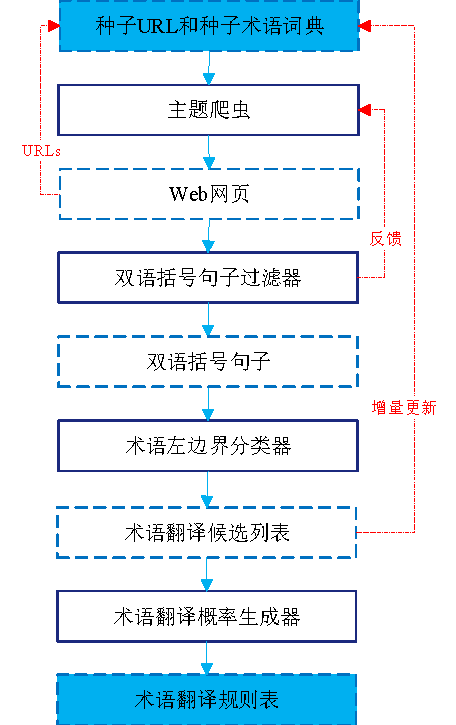
\includegraphics[width=0.6\textwidth]{Figure/Figure_4_4.pdf}
	\caption{互联网术语翻译知识挖掘方法的工作流}
	\label{Fig_term_extract_workflow}
\end{figure}

在本节中,为了从双语括号句子中抽取准确率比较高的术语翻译知识,我们提出一个简单但有效的互联网术语翻译知识抽取方法,主要包括四个部分:

(1)有选择地抓取含有双语括号句子网页的主题爬虫。不同于通用爬虫,本文的主题爬虫尽可能避免抓取不含双语括号句子的网页。在访问某个URL之前,需要预测该URL对应的网页中包含双语括号句子的概率。

(2)获取包含双语术语对的双语括号句子过滤器。网页中的括号有多种用途,如术语翻译、解释、补充、举例等。因此,过滤器的任务是挑选出包含双语术语翻译对的带括号的句子,并向主题爬虫反馈当前URL对应的网页的双语括号句子的分布情况。

(3)从双语括号句子中抽取双语术语翻译知识的术语左边界分类器。该分类器使用预先训练好的最大熵模型对目标术语的左边界进行识别,然后将识别出的左边界作为锚点,通过左右扩展而生成术语翻译候选列表。最大熵模型的训练语料为包括维基百科在内的自然标注语料和种子词典。

(4)术语翻译概率生成器。不同于同类方法,本文并不生成多用途的双语术语表。我们设计了一个术语翻译概率生成器,来生成面向统计机器翻译解码器的术语翻译规则表,从而获得更好的机器翻译自动译文。

基于双语括号句子的术语翻译挖掘方法的工作流如图\ref{Fig_term_extract_workflow}所示。该方法的输入为种子URL和种子术语词典,最终输出为带概率的术语翻译规则表,类似于统计翻译的短语翻译规则表,如示例\ref{Fig_term_extract_workflow}所示。

在工作流中,中间结果包括主题爬虫获取的Web网页和URL,双语括号句子过滤器筛选出的双语括号句子,术语左边界分类器的术语翻译候选列表,以及增量更新后的种子术语词典。

\begin{center}
	\begin{boxedminipage}[h]{0.9\linewidth}
		\small
		\textbf{示例4.2:}
		
		communication ||| 通信 ||| 0.387201 0.358436 0.623309 0.668845 ||| 0-0
		
		interprocess ||| 间 ||| 0.00358423 0.0028275 0.333333 0.6 ||| 0-0
		
		interprocess ||| 进程 间 ||| 0.333333 0.00160575 0.666667 0.24 ||| 0-0 0-1
		
		interprocess communication ||| 间 通信 ||| 0.333333 0.000101348 0.333333 0.401307 ||| 0-0 1-1
		
		interprocess communication ||| 进程 间 通信 ||| 0.4 0.000575558 0.666667 0.160523 ||| 0-0 0-1 1-2
		
		IPC ||| 间 通信 ||| 0.333333 0.416858 0.0454545 0.352726 ||| 0-0 0-1
		
		IPC ||| 进程 间 通信 ||| 0.65625 0.731707 0.5 0.120435 ||| 0-0 0-1 0-2
	\end{boxedminipage}
\end{center}

接下来我们将分别讨论工作流的四个主要部分。其中,关键部分为基于最大熵模型的目标语言术语左边界分类器,以及术语翻译概率生成器。

\subsection{主题爬虫}

对于本文而言,主题爬虫的主要任务是预测要访问的URL对应的网页中包含双语括号句子的概率。URL包含域名、路径等部分,如“https://en.wikipedia.org /wiki/Memory”的域名和路径分别为“en.wikipedia.org”和“/wiki/Memory”。在大规模URL场景下,我们假设一个网页中包含多个双语括号句子的前提一般需要满足下列条件之一:(1)相同域名网页中的双语括号句子比较多;(2)具有相同父路径的网页中的双语括号句子比较多。因此,我们可以由下列公式根据已访问URL的情况来计算未来的URL可能包含双语括号句子的概率:
\begin{equation}
\log p(url) =0.5\times \log \frac{count_{url.domain}}{total_{url.domain}}+ 0.5\times \log \frac{count_{url.parent}}{total_{url.parent}}
\end{equation}
其中$count$表示双语括号句子的数量,$total$表示该网页中所有句子的数量。已访问网页的双语括号句子数量由双语括号句子过滤器给出。

\subsection{双语括号句子过滤器}

网页中括号的作用包括术语翻译、解释、补充、举例等,如示例4.3所示。

\begin{center}
	\begin{boxedminipage}[h]{0.9\linewidth}
		\small
		\textbf{示例4.3:}
		
		\textbf{术语翻译:}
		
		软件开发中的\underline{焦油坑}(the tar pit)可以通过尽责、专业的过程得以避免。
		
		岩石里有种构造叫\underline{夫妻节理}(英文:coupled joints)。
		
		\textbf{解释:}
		
		蓟北:泛指\underline{蓟州、幽州一带}(现在河北省北部地区),是安、史叛军盘踞的地方。
		
		\textbf{补充:}
		
		\underline{艾米莉•狄金森}(1830-1886)是美国文学史上一个伟大的诗人。
		
		\underline{斯巴达克}(杀开一条血路,大喊)不愿做奴隶的人们!起来!
		
		\textbf{举例: }
		
		从图中两组节理面的\underline{锐角}(beta)可计算出该岩石的内摩擦。
		
		转载请注意说明\underline{来源}(www.qq.com) 
		
		没有被收录在词表中的词,包括各类\underline{专有名词}(人名、地名、企业名等)。
	\end{boxedminipage}
\end{center}

双语括号句子过滤器的主要任务就是识别出用于术语翻译的括号。给定包含括号的句子$s=\ldots c_1c_2\ldots c_n(e_1e_2\ldots e_m) \ldots $,我们通过种子术语词典、括号里外字串的共现频率和预先定义的括号筛选规则来计算句子$s$是双语括号句子的概率:
\begin{equation}\label{bilingual_sent}
\log p(s) = \lambda_1 \log p(domain) + \lambda_2 \log p(page) + \lambda_3 \log r(s) + \lambda_4 \log co(s)
\end{equation}
其中, $p(page)$表示根据该页面的已处理句子预测出的$s$是双语括号句子的概率,$\lambda_1$~$\lambda_4$表示各部分权重参数。

公式\ref{bilingual_sent}中,$r(s)$表示根据种子词典,括号内与括号左边的词匹配成功的比例,计算公式如下:
\begin{equation}
\begin{aligned}
r(s) &= \frac{1}{m} \times \sum_{j=1}^{m} sign(e_j) \\
sign(e_j) & = \left \{
\begin{array}{ll}
0 & \quad \forall \ target' \in dictionary(e_j),\ target' \notin \{c_n\}  \\
1 & \quad \exists \ target' \in dictionary(e_j),\ target' \in \{c_n\}
\end{array}
\right.
\end{aligned}
\end{equation}
其中,$dictionary(e_j)$表示源语言词 在种子词典中的目标语言词集合。
公式\ref{bilingual_sent}中,$co(s)$表示括号左边与括号内的词的平均共现概率:
\begin{equation}
co(s) = \frac{1}{2m} \times \sum_{j=1}^{m} \max_{1\le i \le n, e_j \in s, c_i \in s} \frac{count(e_j, c_i)}{count(e_j)+count(c_i)}
\end{equation}

经过大量的实例分析,我们发现双语术语对有明显的汇集现象,即某些网站或者网页的双语术语对的数量明显多余其它网页,如百科类网站、技术类网页、普通网站的知识性栏目等。如果在一个网页中已发现有大量的双语括号句子中包含置信度比较高的双语术语对,那么该网页中剩下的带括号的句子也有很大概率是双语括号句子。这些先验信息有助于提高识别双语括号句子的准确率。因此,公式\ref{bilingual_sent}中的$p(page)$表示根据该页面已过滤的句子预测出的双语括号句子的概率,推导公式如下:
\begin{equation}
s(page) = \frac{1}{|page|} \sum_{s'\in page}\left( \frac{\lambda_3}{\lambda_3 + \lambda_4}\times r(s') + \frac{\lambda_4}{\lambda_3 + \lambda_4}\times co(s') \right)
\end{equation}
其中,$|page|$表示该页面已解析的所有句子的数目。

类似地,公式4.13中的$p(domain)$表示根据该域名已访问的网页预测出的双语括号句子的频率,推导公式如下:
\begin{equation}
s(domain) = \frac{1}{|domain|} \sum_{s'\in domain}\left( \frac{\lambda_3}{\lambda_3 + \lambda_4}\times r(s') + \frac{\lambda_4}{\lambda_3 + \lambda_4}\times co(s') \right)
\end{equation}
其中,$|domain|$表示该域名下已经解析的句子数。

需要提及的是,对于$\log p(s)$值低于阈值的句子,但按预先定义的规则又可能是双语括号句子的情形时,我们暂时将句子$s$标记为负例。待该域名下已解析的句子数达到设定的阈值时,再重新计算该句子的$\log p(s)$。

在本文中,$\lambda$的默认值分别为:$\lambda_1 = \lambda_2 = 0.2$,$\lambda_3 = \lambda_4 =0.3$。

\subsection{术语左边界分类器}

\begin{figure}[!bt]
	\centering
	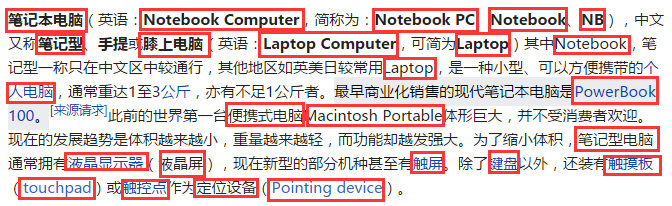
\includegraphics[width=0.9\textwidth]{Figure/Figure_4_5.png}
	\caption{用以训练术语左边界分类器的自然标注语料。红框为人工标注}
	\label{Fig_term_left_trainning}
\end{figure}

为了抽取出双语术语候选,关键任务是识别出目标语言术语的左边界。然而,基于统计的术语识别方法为了提高准确率导致在一些领域只有非常低的召回率,如基于对数似然[Cohen, 1995; Lefever et al., 2009]、TF-IDF [Evans and Lefferts, 1995; Medelyan and Witten, 2006]、C-value/NC-value [Frantzi and Ananiadou, 1999]和其它方法[Ahmad et al., 2000; Park et al., 2002; Kozakov et al., 2004; Sclano and Velardi, 2007; Zhou et al., 2008; Zhang et al, 2008a; Kostoff et al., 2009]。更糟糕的是,一些基于频率阈值的方法减少了算法的搜索空间,导致很多低频术语被错误地过滤掉。

为了挖掘出更多的低频术语,我们需要提高召回率,我们将自然标注语料作为训练语料来适应比较宽泛的领域。最后,我们用图\ref{Fig_term_left_trainning}所示的维基百科语料来训练基于最大熵模型的术语左边界分类器。图\ref{Fig_term_left_trainning}中,自然标注(粗体、超链接等)与红框所示人工标注的术语有较大部分是重合的,因此可以作为术语左边界分类器的训练语料。因此我们通过一些简单规则过滤后直接将自然标注转换为术语左边界分隔符,然后作为术语左边界分类器的训练语料。

在本文中,我们为术语左边界分类器的最大熵模型设计了如下特征:最靠近术语之前的四个词$W_{s-4}, \ldots, W_{s-1}$及对应的词性$POS_{s-4}, \ldots, POS_{s-1}$;紧跟术语之后的四个词$W_{s+1}, \ldots, W_{s+4}$及对应的词性$POS_{s+1}, \ldots, POS_{s+4}$;术语的第一个词$WL$及其词性$POSL$;术语最后一个词$WR$及其词性$POSR$;根据种子术语词典,术语中的词与括号里的源语言术语匹配的词的百分比$D$。

当输入一个双语括号句子后,术语左边界分类器的输出是括号左边最可能的术语左边界$c_i$及其概率$p(c_i)$。目标语言词$c_i)$包括在术语中,即术语的第一个词。至此,我们可以抽取出如表\ref{Table_dict_samples}所示的双语术语候选,将其中$p(c_i)$超过阈值的双语术语对添加到种子术语词典中。

\begin{table}[!hbt]
	\centering
	\begin{tabular}{l|l}
		\hline
		源语言 & 目标语言     \\ \hline
		Mihr-Ohrmazd & 拂多诞      \\ 
		Wicca & 威卡尔      \\ 
		Francis Dashwood & 弗朗西斯达希武德 \\ 
		Religious Studies & 宗教学      \\ 
		Introduction to the Science of Religion & 宗教科学引论   \\
		History of Religions & 宗教史学     \\ 
		Phenomenology of Religion & 宗教现象学    \\
		anomalous monism & 无法则一元论   \\ 
		qualia & 感质       \\ 
		Panspermia & 泛种论      \\ 
		Determinism & 决定论      \\ \hline
	\end{tabular}
	\caption{根据术语左边界分类器结果抽取出的双语术语候选}
	\label{Table_dict_samples}
\end{table}

\subsection{术语翻译概率生成器}

为了显著提升统计机器翻译自动译文质量,我们并不直接将上一步骤中抽取的双语术语候选提供给统计机器翻译解码器直接查询,而是根据术语候选的上下文信息,让术语翻译概率生成器生成与翻译模型类似的含翻译概率的术语翻译表。结合术语左边界分类器给出的左边界候选n-best生成最终的术语翻译概率。因此,最佳左边界$c_i$的搜索过程可以形式化为如下联合模型:
\begin{equation}\label{term_extract_joint}
i= \argmax_{1 \le i \le n} \left[ p(c_i)^{\lambda_5} \times p(c_i\ldots c_n|e_1\ldots e_m)^{\lambda_6} \times p(e_1\ldots e_m|c_i\ldots c_n)^{\lambda_7} \right]
\end{equation}
其中,$p(c_i\ldots c_n|e_1\ldots e_m)$和$p(e_1\ldots e_m|c_i\ldots c_n)$表示词汇化翻译概率。

在示例4.1中,$s=$“所以 只能 使用 进程 间 通讯(interprocess communication,IPC)”。因此,对于源语言术语“interprocess communication”,$c_1=$“所以”,$c_2=$“只能”,$c_3=$“使用”,$c_4=$“进程”,$c_5=$“间”,$c_6=$“通讯”,$e_1=$“interprocess”,$e_2=$“communication”。我们的基线系统是用维基百科语料训练的基于最大熵的术语识别分类器,它给出的左边界识别结果为$c_5$,即目标术语为$c_5c_6=$“间 通讯”。为了减小基线系统的识别错误带来的负面影响,我们将$c_5$作为锚点,建立滑动窗口,进而扩展或者收缩左边界生成新的目标术语候选列表,其中就包括正确的目标语言术语$c_4c_5c_6=$“进程 间 通信”。然后,我们利用公式式\ref{term_extract_joint},通过求解最大的联合概率值来找到最佳的目标语言术语“进程 间 通信”。在本文中,公式\ref{term_extract_joint}中的词汇化翻译概率通过基于隐马尔可夫的词对齐模型计算得到。

基于上述结果,我们可以抽取出术语翻译规则,并生成如示例4.2所示的带翻译概率的术语翻译表。在示例4.2中,如“communication ||| 通信 ||| 0.387201 0.358436 0.623309 0.668845 ||| 0-0”包含七个部分,分别是源语言术语、目标语言术语、正向短语翻译概率、正向词汇化翻译概率、反向短语翻译概率、反向词汇化翻译概率和术语词对齐。这与基于短语的翻译模型一致,有利于统计机器翻译解码器的信息融合。

在本文中,$\lambda_5$、$\lambda_6$和$\lambda_7$的默认值分别为0.4,0.3和0.3。

\section{基于术语识别边界信息的统计翻译术语解码方法}

如前文所述,人名、地名、机构名等命名实体有明显的边界特征,相对容易进行识别与对齐。一般而言,将命名实体直接翻译方法用于统计翻译解码器就可以取得比较好的翻译效果。在这里,“直接翻译”意味着:(1)在预处理阶段,将识别出来的命名实体直接替换为对应标签,如将人名替换为“PERSON”,将地名替换为“LOC”,将机构名替换为“ORG”;(2)在后处理阶段,将标签替换为对应命名实体的译文。

但是,用与翻译命名实体的方式“直接翻译”术语并不能明显改善机器翻译自动译文的质量。最主要的原因就是目前的术语识别模型还不够好,识别准确率大幅弱于命名实体识别。另外,由于术语本身是与领域高度相关的,为目标领域训练高性能的术语识别分类器需要大量高质量且同领域的人工标注训练语料,这进一步加大了术语识别的难度。在这种情况下,如果将识别出的术语直接替换为标签,然后通过查询大规模双语术语词典的方式来翻译术语,则会出现大量的匹配错误。另一个重要的原因在于,术语翻译存在大量的一对多现象,所以术语翻译就可能会受到上下文的影响。如在IT领域,“type”可能是“型号”,也可能是“字体”(type face),目标译文需要根据具体上下文确定。而在大多数情况下,命名实体的翻译是可以独立于上下文的。

在本文中,为了更好地将术语翻译融入到统计机器翻译的流程中,我们提出了不严格区分术语词与非术语词的,融合术语识别边界信息的统计翻译术语解码方法。该方法区别于“直接翻译”的关键在于,后者先识别并用标签替换,然后通过独立查表或者搜索的方式获得术语翻译,而前者是在识别的基础上根据上下文确定最终译文。

为了避免“直接翻译”方法在术语翻译任务上的缺陷,为了将术语翻译嵌入到人机交互式机器翻译系统中,我们提出的统计翻译术语解码方法尝试回答两个问题:(1)抽取什么样的术语翻译知识;(2)如何将术语翻译与机器翻译系统结合起来提高自动译文质量。主要思想是在人机交互式机器翻译系统中,先抽取多种类型的术语翻译知识,再优化统计机器翻译解码器的术语处理过程。

\subsection{抽取多种类型的术语翻译知识}

为了将术语翻译知识与统计翻译模型相融合,在词对齐任务完成之后、抽取术语翻译知识之前,术语开始/结束标签和术语对齐标志将被插入最终的词对齐结果中。除了常规的短语翻译规则之外,我们还要抽取另外四种包含术语标签的翻译规则,依泛化程度由低到高排列,分别为:含术语标签的翻译规则、双语术语对、含术语槽的翻译规则和术语翻译模版。另外,术语开始/结束标签必须成对出现在翻译规则中。为简洁起见,图\ref{Fig_term_knowledge_sample}列出了从图\ref{Fig_joint_term_overview}的双语句对中抽取出的术语有关的翻译知识。

\begin{figure}[!bt]
	\centering
	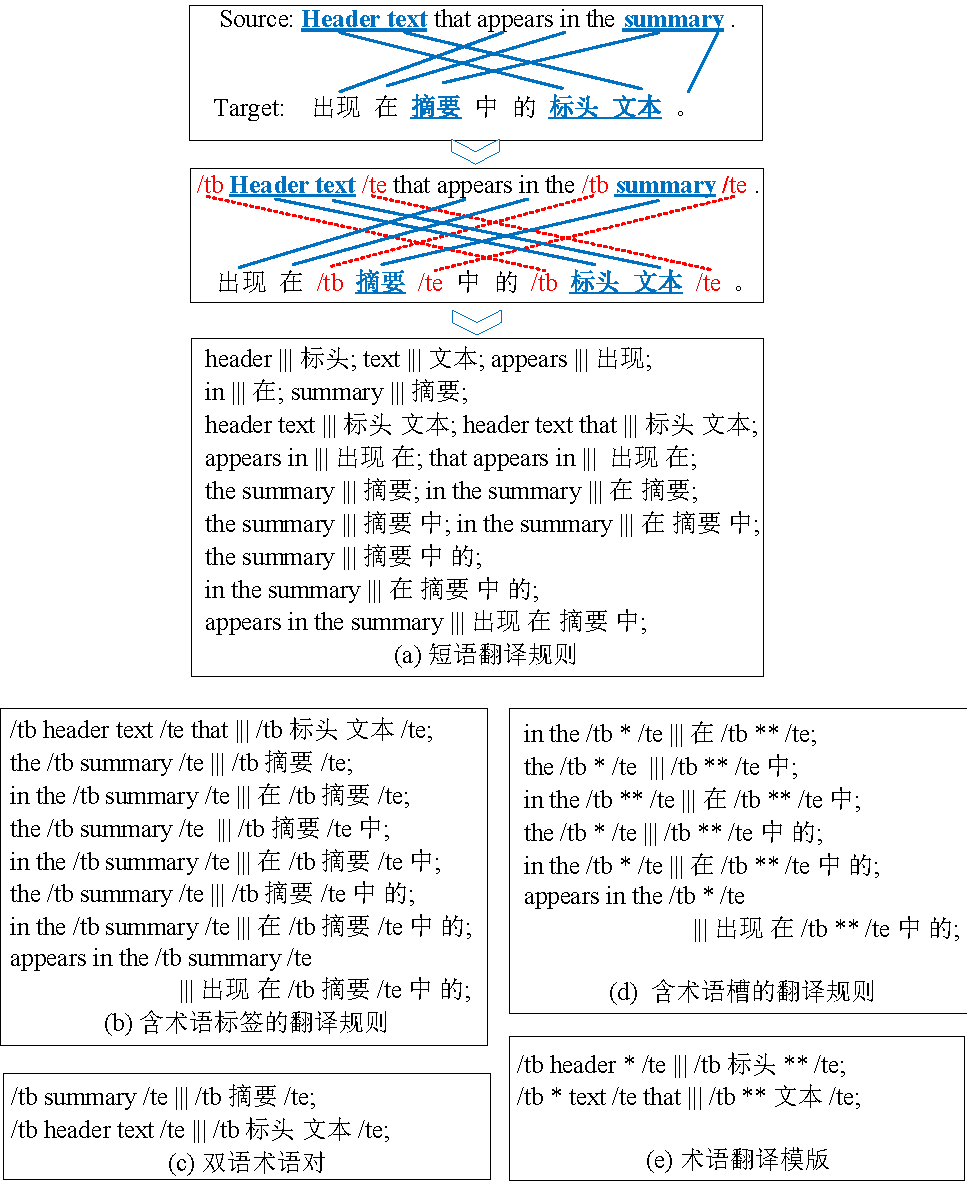
\includegraphics[width=0.95\textwidth]{Figure/Figure_4_6.pdf}
	\caption{抽取出的术语翻译知识示例}
	\label{Fig_term_knowledge_sample}
\end{figure}

如图\ref{Fig_term_knowledge_sample}所示,从四阶段联合模型的结果中直接抽取出的如图\ref{Fig_term_knowledge_sample}(c)所示的双语术语对和如图\ref{Fig_term_knowledge_sample}(e)术语翻译模版没有上下文信息。由于术语翻译模版在缺乏上下文信息的情况下进行泛化,因此术语翻译模版的翻译风险最高。相对应的,如图\ref{Fig_term_knowledge_sample}(d)所示的含术语槽的翻译规则的翻译风险次之。而如图\ref{Fig_term_knowledge_sample}(b)所示的含术语标签的翻译规则最可靠,因为同时抽取了上下文和完整的双语术语。

对于抽取出的术语翻译知识,都需要计算如示例4.2所示的Moses风格的四种特征值:正向短语翻译概率$\phi (\overline{t}|\overline{s})$、正向词汇化翻译概率$lex(\overline{t}|\overline{s})$、反向短语翻译概率$\phi (\overline{s}|\overline{t})$和反向词汇化翻译概率$lex(\overline{s}|\overline{t})$。例如,令$count(\overline{s}, \overline{t})$指双语短语对的共现频次,$p(t_i|s_j)$指源语言词到目标语言词的翻译概率,则正向词汇化翻译概率和反向短语短语翻译概率可分别由公式\ref{staight_lex_prob}和\ref{reverse_phrase_prob}计算得到:

\begin{equation}\label{staight_lex_prob}
\phi (\overline{s}|\overline{t}) = \frac{count(\overline{s}, \overline{t})}{\sum_{\overline{s_i}} count(\overline{s}, \overline{t})}
\end{equation}

\begin{equation}\label{reverse_phrase_prob}
lex(\overline{t}|\overline{s}, a) = \prod_{i=1}^{length(\overline{t})} \frac{1}{|j|(i,j) \in a|} \sum_{\forall (i,j) \in a} p(t_i|s_j)
\end{equation}

\subsection{优化统计机器翻译解码器}

抽取出术语翻译知识之后,对于统计机器翻译解码器而言,最重要的任务是在解码过程中能兼容术语识别错误。为了更有效地将术语翻译知识融合到统计机器翻译解码器中,我们提出了两点优化方法:(1)为了适应不同程度的泛化风险而引入了四个额外的术语翻译有关的权重参数;(2)为了兼容识别错误而采用术语识别分类器的前N个锚点候选。

首先,为了适应泛化风险而引入的四个权重参数,即$\lambda_b$、$\lambda_c$、$\lambda_d$ 和$\lambda_e$,分别对应含术语标签的翻译规则、双语术语对、含术语槽的翻译规则和术语翻译模版的权重。同其它模型的权重参数一样,$\lambda_b$~$\lambda_e$的值在最小错误率训练中确定。

其次,在翻译过程中,对于源语言术语识别,我们选取分类器给出的前3个术语锚点。即$N$的默认值为3。经过我们的尝试发现,过大的$N$值并不会明显改善最终的翻译质量,但会大幅降低机器翻译解码器的解码速度。

上述提出的优化方法不但结合了直接翻译方法的优点,如引入的双语术语对和含术语槽的翻译规则分别对应双语命名实体词典和标签替换与还原,而且对术语识别错误还有很好的兼容能力。

\section{实验}

\subsection{实验数据}

本文将通过英中翻译来测试融合术语识别边界信息的术语翻译方法的性能。

机器翻译系统的训练集包含1,199,589句平行句对,人工标注了词对齐和术语结果的测试集包含1,100句,用作最小错误率训练的开发集为1,000句,均随机抽样于微软本地化翻译记忆语料库。初始化术语识别分类器的训练数据为1,133,913对英中双语维基百科词条标题。种子术语词典中不仅包含102,308个源语言词的网络词典(http://www.mdbg.net/chindict/chindict.php?page=cc-cedict)和24,094个汉字的中文拼音表(http://www.51windows.net/pages/gb2312. htm),还包括从微软术语库抽取的24,094对英中术语。基于隐马尔可夫模型的术语词对齐模型的训练语料为1,133,913对英中双语维基百科词条标题和微软术语库抽取的24,094对英中术语。

\subsection{实验设置}

本文使用我们实现的一套统计机器翻译工具集作为翻译性能的测试框架。这套工具集包括术语识别、术语对齐、词对齐和短语翻译表抽取。其中,翻译模型为基于最大熵模型的短语翻译模型[Xiong et al., 2006]。分别使用SRI语言模型训练工具[Stolcke, 2002]训练基于修正的Kneser-Ney平滑的语言模型,使用ZMERT[Zaidan, 2009]进行最小错误率训练[Och, 2003]来调节参数权重,大小写敏感的BLEU-4[Papineni et al., 2002]评估标准去评价机器翻译的译文质量。所有方法的机器翻译系统所使用的训练集、开发集和测试集均分别完全一致。

我们使用准确率(P)、召回率(R)和F值(F)来评价术语识别与词对齐质量,使用准确率来评价术语级翻译质量(P),使用大小写敏感的BLEU-4评估标准来评价句子级翻译质量。统计显著性检验使用重采样方法[\cite{Koehn:2004b}]。

\subsection{融合双语术语识别的联合词对齐方法的实验结果}

\textbf{(1)单语术语识别}

首先,我们比较不同的联合阶段对术语识别性能的影响。相关方法的英语和中文的术语识别实验结果分别标为“En-Baseline”、“Ch-Baseline”、“En-Joint-C-Stage”、“Ch-Joint-C-Stage”、“En-Joint-D-Stage”和“Ch-Joint-D-Stage”。“*-Baseline”指基线系统,即分别独立执行各阶段。“*-C-Stage”表示仅术语识别与双语术语对齐联合执行。“*-D-Stage”表示本文提出的四阶段联合模型。“En-*”和“Ch-*”分别表示英中单语术语识别结果。表\ref{Table_term_recognition_result}给出了不同方法的术语识别性能结果。“**”表示比基线系统在置信区间$p<0.01$显著提高。

\begin{table}[!htbp]
	\centering
	\begin{tabular}{|l|c|c|c|}
		\hline 
		方法  & P/\% & R/\% & R/\% \\ \hline
		En-Baseline      & $62.94$ & $65.61$ & $64.25$ \\ \hline
		En-Joint-C-Stage & $67.35$ & $71.47$ & $69.34$ \\ \hline
		En-Joint-D-Stage & $71.20^{**}$ & $76.84^{**}$ & $\mathbf{73.91^{**}}$ 
		\\ \hline
		Ch-Baseline      & $57.21$ & $66.67$ & $61.58$ \\ \hline
		Ch-Joint-C-Stage & $65.13$ & $74.86$ & $69.65$ \\ \hline
		Ch-Joint-D-Stage & $67.89^{**}$ & $75.03^{**}$ & $\mathbf{71.28^{**}}$ \\
		\hline
	\end{tabular}
	\caption{术语识别性能结果}
	\label{Table_term_recognition_result}
\end{table}

根据图\ref{Table_term_recognition_result}中的实验结果,我们可以发现初始化术语识别结果可以作为非常有用的锚点以进一步进行术语识别,因而单语术语识别的F值绝对值被显著提升了超过9.66个百分点。根据表\ref{Table_term_recognition_result}中的粗体字,我们可以知道,术语识别与词对齐融合后,单语术语识别的性能可以得到显著提高。

\textbf{(2)双语术语对齐}

其次,我们比较不同的联合阶段对双语术语对齐性能的影响。“Baseline”指用流水线方法的基线系统,即各阶段分别独立执行。基线系统首先进行源语言和目标语言的单语术语识别,然后直接将术语结果作为约束进行双语术语对齐,后续阶段不与之前的阶段进行交互。测试数据的双语术语对齐标准答案由人工标注给出。“Joint-C-Stage”表示仅术语识别与双语术语对齐联合执行。“Joint-D-Stage”表示本文提出的四阶段联合模型。表\ref{Table_term_alignment_result}给出了不同方法的双语术语对齐性能结果。“**”表示比基线系统在置信区间$p<0.01$显著提高。

根据表\ref{Table_term_alignment_result}中的实验结果,将术语识别、双语术语对齐与词对齐融合之后,双语术语对齐的F值绝对值被显著提升了8.25个百分点。由此可见,双语术语对齐与词对齐融合之后,双语术语识别的性能可以得到显著提高。

\begin{table}[!htbp]
	\centering
	\begin{tabular}{|l|c|c|c|}
		\hline
		方法  &  P/\% &  R/\% &  R/\% \\
		\hline
		Baseline      & $49.38$ & $56.41$ & $52.66$ \\ \hline
		Joint-C-Stage & $53.47$ & $59.44$ & $56.29$ \\ \hline
		Joint-D-Stage & $58.29^{**}$ & $63.78^{**}$ & $\mathbf{60.91^{**}}$ \\
		\hline
	\end{tabular}
	\caption{双语术语对齐性能结果}
	\label{Table_term_alignment_result}
\end{table}

\textbf{(3)词对齐}

接下来,我们将评估不同的联合阶段对词对齐性能的影响。我们有三个基线系统,分别为GIZA++、单独的基于隐马尔可夫模型的词对齐系统和流水线方法实现的基于隐马尔可夫模型的词对齐系统,分别被标记为“GIZA++”、“Baseline-1”和“Baseline-2”。三个基线系统均采用流水线方法,即首先进行源语言和目标语言的单语术语识别,然后直接将术语结果作为约束进行双语术语对齐,然后将双语术语对齐结果作为双语词对齐的约束条件。“Joint-C-Stage”表示仅术语识别与双语术语对齐联合执行,然后单独进行词对齐。“Joint-D-Stage”表示本文提出的四阶段联合模型。在本文中,我们使用F值[\cite{Fraser:2007,LiuYang:2010}]作为词对齐性能的评价指标。表\ref{Table_word_alignment_result}给出了不同方法的双语词对齐性能结果。“**”表示比基线系统在置信区间$p<0.01$显著提高。

\begin{table}[!htbp]
	\centering
	\begin{tabular}{|l|c|c|c|}
		\hline
		方法  &  P/\% &  R/\% &  R/\% \\
		\hline
		GIZA++        & $69.28$ & $75.83$ & $72.41$ \\ \hline
		Baseline-1    & $67.06$ & $73.18$ & $69.99$ \\ \hline
		Baseline-2    & $64.47$ & $70.62$ & $67.41$ \\ \hline
		Joint-C-Stage & $69.45$ & $76.49$ & $72.80$ \\ \hline
		Joint-D-Stage & $71.19^{**}$ & $78.51^{**}$ & $\mathbf{74.67^{**}}$ \\
		\hline
	\end{tabular}
	\caption{双语词对齐性能结果}
	\label{Table_word_alignment_result}
\end{table}

表\ref{Table_word_alignment_result}中的基线系统“GIZA++”启用了IBM模型1-5和基于隐马尔可夫的词对齐模型,同时还包括GIZA++已实现的优化措施。另外两个基线系统“Baseline-1”和“Baseline-2”均为独立的基于隐马尔可夫的词对齐模型。因此,根据表\ref{Table_word_alignment_result},基线系统“Baseline-1”的词对齐性能明显弱于GIZA++,这说明流水线方法并不能改善词对齐性能,因为现有单语术语词识别的性能过低。根据表\ref{Table_word_alignment_result}中的粗体字,双语术语对齐与词对齐融合之后,相比基于隐马尔可夫模型的基线系统,代表词对齐性能的绝对F值提高了4.68个百分点。即便与GIZA++相比,四阶段联合模型的词对齐性能也提高了2.26个绝对F值百分点。

\textbf{(4)机器翻译}

最后,我们将测试提出的四阶段联合模型是否能提高最终的机器翻译自动译文质量,包括术语级和句子级的翻译质量。我们有三个基线系统,分别为Moses、我们实现的基于最大熵模型的短语翻译模型的翻译系统和考虑术语翻译的流水线方法实现的翻译系统,分别被标记为“Moses”、“Baseline-1”和“Baseline-2”。其中,Moses未考虑术语翻译,使用了GIZA++作为词对齐工具。基线系统“Baseline-2”在基线系统“Baseline-1”的基础上加入了术语处理环节。“Baseline-1”和\linebreak
“Baseline-2”使用基于隐马尔可夫模型的词对齐工具。 “Joint-C-Stage-Direct”表示术语识别与双语术语对齐联合执行,然后单独进行词对齐,最后抽取短语翻译规则。“Joint-D-Stage-Direct”表示采用本文提出的四阶段联合模型进行词对齐,最后抽取短语翻译规则。在测试阶段,“*-Direct”表示机器翻译解码器采用的是通过查询双语术语表的直接翻译术语的方法。我们使用准确率来评价术语翻译质量(P),即只有当目标术语完全正确的情况下才认为源语言术语被正确翻译。使用不区分大小写的BLEU-4来评价句子的翻译质量。表\ref{Table_joint_term_mt_result}给出了不同方法的机器翻译性能结果。“**”表示比基线系统在置信区间$p<0.01$显著提高。

\begin{table}[!htbp]
	\centering
	\begin{tabular}{|l|c|c|}
		\hline
		方法  & 术语/P/\% & 句子/BLEU\% \\ 
		\hline
		Moses         & 87.30 & 63.58 \\ \hline
		Baseline-1    & 86.53 & 63.09 \\ \hline
		Baseline-2    & 78.43 & 62.68 \\ \hline
		Joint-C-Stage+Direct & 87.73 & 63.54 \\ \hline
		Joint-D-Stage+Direct & $\underline{91.04^{**}}$ & $\underline{63.96^{**}}$ \\
		\hline
	\end{tabular}
	\caption{机器翻译性能结果}
	\label{Table_joint_term_mt_result}
\end{table}

根据表\ref{Table_joint_term_mt_result}的实验结果,我们可以发现在相同的数据集上,我们实现的机器翻译系统“Baseline-1”的性能弱于Moses,需要改进包括词对齐在内的一系列基础工具集。引入流水线的术语翻译方法之后,不论是术语翻译质量还是句子翻译质量都有比较明显的下降。同时表明,流水线方法并不能改善机器翻译性能,因为现有单语术语词识别的性能过低,不同阶段之间的错误传递严重影响最终的机器翻译性能。但是,“Joint-C-Stage-Direct”的实验结果表明,仅术语识别与双语术语对齐联合执行,然后单独进行词对齐,也能改善术语和句子的翻译质量,最后与Moses的实验结果达到可比的程度。

根据表\ref{Table_joint_term_mt_result}“Joint-D-Stage-Direct”的实验结果,我们可以发现,本文提出的四阶段联合模型将术语翻译质量显著提高了超过4.5的绝对百分比,同时也显著优于Moses的术语翻译结果。改善了术语翻译质量之后,整句的翻译质量也会得到提升。在句子翻译质量方面,四阶段联合模型提升了0.87个绝对BLEU值的百分点。受限于直接翻译术语的方法,我们并没有充分利用从平行句对中抽取的术语翻译知识。因此,句子翻译质量的提升尽管达到了统计显著的水平,但应该还有较大的上升空间。

\subsection{基于双语括号句子的术语翻译挖掘方法的实验结果}

\textbf{(1)术语翻译挖掘}

首先,我们将评估基于双语括号句子的术语翻译挖掘方法在抽取网络术语翻译知识方面的性能。在我们的实验中,主题爬虫已经下载了162,543,832个页面,其中,12,673,286个网页共包含49,976,931个双语括号句子。基线系统被标记为“Baseline”,是根据文献[\cite{Cao:2007}]实现的从大规模单语网页中挖掘双语词典的系统,从这些双语括号句子中共抽取出10,823,132对双语术语。我们在本文中提出的基于双语括号句子的术语翻译挖掘方法的系统被标记为“TermExt”,从相同的双语括号句子中抽取出12,048,310对双语术语。然后对各自抽取出的术语对进行有放回的随机抽样10次,每次抽样1000对术语。每次抽样后,统计中文术语准确率和术语对准确率。待10次抽样完成,分别计算中文术语准确率和术语对准确率的平均值。中文术语准确率指双语括号左边的目标语言单语术语识别正确率。术语对准确率是指抽取出的短语对经人工确认为双语术语对的百分比。表\ref{Table_bilingual_term_extract_result}给出了完整的双语术语抽取性能结果。“**”表示比基线系统在置信区间$p<0.01$显著提高。

\begin{table}[!htbp]
	\centering
	\begin{tabular}{|l|c|c|c|}
		\hline
		方法  & 术语对总数 & 中文术语准确率 & 术语对准确率 \\ 
		\hline
		Baseline         & 10,823,132 &	94.30 &	88.20 \\ \hline
		TermExt	         & 12,048,310 &	\textbf{97.20**} &	\textbf{92.30**} \\
		\hline
	\end{tabular}
	\caption{双语术语抽取性能结果}
	\label{Table_bilingual_term_extract_result}
\end{table}

根据表\ref{Table_bilingual_term_extract_result}的实验结果,相对于基线系统,我们提出的术语翻译挖掘方法比基线系统多抽取出11.32\%的术语对,中文术语即目标语言术语识别的准确率提高了2.9个绝对百分点,术语对准确率提升了4.1个绝对百分点,且均通过统计显著性检验。因此,我们可以认为提出的基于双语括号句子的术语翻译挖掘方法确实大幅提升了术语翻译挖掘的性能。

\textbf{(2)机器翻译}

接下来,我们将评估用不同挖掘方法和不同的术语翻译知识融合方法是否能提高最终的机器翻译自动译文质量,包括术语级翻译质量和句子级的翻译质量。在机器翻译实验中,我们有两个基线系统,分别为Moses、我们实现的基于最大熵模型的短语翻译模型的翻译系统,分别被标记为“Moses”、“MaxEntSMT”。基线系统均未考虑术语翻译问题。“*Dict”表示在我们实现的机器翻译系统中,机器翻译解码器采用的是通过查询双语术语表的直接翻译术语的方法。“BaselineDict” 表示由基线系统“Baseline”,即根据文献[\cite{Cao:2007}]实现的系统,抽取的双语术语表。“TermExtDict”表示由“TermExt”,即本文提出的基于双语括号句子的术语翻译挖掘方法实现的系统,抽取出的双语术语表。其中,“TermExtDict”为术语左边界分类器的输出结果,即未经术语翻译概率生成器处理。而“TermExtTable”为术语翻译概率生成器的输出结果。即,“*Table”表示机器翻译解码器采用的是术语柔性翻译方法,其它实验设置与“*Dict”完全一致。表\ref{Table_term_extract_mt_result}给出了完整的机器翻译性能结果。“**”表示比基线系统在置信区间$p<0.01$显著提高,“*”表示比基线系统在置信区间$p<0.05$显著提高。

\begin{table}[!htbp]
	\centering
	\begin{tabular}{|l|c|c|}
		\hline
		方法  & 术语/P/\% & 句子/BLEU\% \\ 
		\hline
		Moses         & 87.30 & 63.58 \\ \hline
		MaxEntSMT	  & 86.53 &	63.09 \\ \hline
		MaxEntSMT+BaselineDict & 89.47 & 63.76 \\ \hline
		MaxEntSMT+TermExtDict &	91.22** &	63.91* \\ \hline
		MaxEntSMT+TermExtTable & \textbf{94.38**} &	\textbf{64.84**} \\
		\hline
	\end{tabular}
	\caption{不同双语术语知识挖掘和融合方法的机器翻译性能结果}
	\label{Table_term_extract_mt_result}
\end{table}

在表4.7的实验结果数据中,与“BaselineDict”直接可比的结果是\linebreak
“TermExtDict”,因为前者并无生成术语翻译规则表的算法。使用直接翻译术语的方法,通过“MaxEntSMT+BaselineDict”与“MaxEntSMT+TermExtDict”的结果对比我们可以发现,我们提出的基于双语括号句子的术语翻译挖掘方法,如果没有术语翻译概率生成器,那么在术语翻译准确率方面可以提升超过1.5个绝对百分点,在句子翻译性能方面可以提升的BLEU值为0.15个绝对百分点。虽然均通过$p<0.05$的显著性检验,但优势并不明显。

而表\ref{Table_term_extract_mt_result}中的粗体字表明,在术语翻译概率生成器和术语柔性翻译方法的帮助下,我们提出的基于双语括号句子的术语翻译挖掘方法,在术语翻译准确率方面可以提升约6个绝对百分点,在句子翻译性能方面可以提升的BLEU值超过1个绝对百分点,且均通过$p<0.01$的显著性检验。

因此,通过实验结果,我们可以认为:基于双语括号句子的术语翻译挖掘方法确实能提高双语术语抽取性能,且与术语柔性翻译方法结合后,能显著提升最终统计机器翻译的术语和句子翻译质量。


\subsection{基于术语识别边界信息的统计翻译术语解码方法的实验结果}

在本小节中,将结合具体案例来评估融合术语识别边界信息的统计翻译术语解码方法对机器翻译译文质量的影响。通过上一节的实验,我们已经知道使用术语柔性翻译方法可以将从网络上挖掘到的术语翻译知识更好地融合到统计机器翻译系统中。因此,在本小节中,我们以四阶段联合模型抽取出的翻译知识为例,分析术语柔性翻译方法是如何影响最终的自动译文的质量。在表\ref{Table_joint_term_mt_result}的基础上,我们加入融合术语识别边界信息的统计翻译术语解码方法的性能结果,表\ref{Table_soft_direct_result}给出了完整的性能结果。其中,“*-Soft”表示机器翻译解码器采用的是融合术语识别边界信息的统计翻译术语解码方法,其它实验设置与“*-Direct”完全一致。“**”表示比基线系统在置信区间$p<0.01$显著提高。

\begin{table}[!htbp]
	\centering
	\begin{tabular}{|l|c|c|}
		\hline
		方法  & 术语/P/\% & 句子/BLEU\% \\ 
		\hline
		Moses         & $87.30$ & $63.58$ \\ \hline
		Baseline-1    & $86.53$ & $63.09$ \\ \hline
		Baseline-2    & $78.43$ & $62.68$ \\ \hline
		Joint-C-Stage+Direct & $87.73$ & $63.54$ \\ \hline
		Joint-C-Stage+Soft & $90.32$ & $63.91$ \\ \hline
		Joint-D-Stage+Direct & $\underline{91.04^{**}}$ & $\underline{63.96^{**}}$ \\ \hline
		Joint-D-Stage+Soft & $\mathbf{94.87^{**}}$ & $\mathbf{65.24^{**}}$ \\
		\hline
	\end{tabular}
	\caption{术语柔性翻译方法与直接翻译方法的性能结果对比}
	\label{Table_soft_direct_result}
\end{table}

根据表\ref{Table_soft_direct_result}的实验结果,我们可以发现基于术语识别边界信息的统计翻译术语解码方法大幅提高了术语和句子的翻译质量。相对于基线系统Moses而言,术语翻译准确率被提高了超过7.5的绝对百分点,句子翻译的BLEU值被提升了超过1.6个绝对百分点,且均通过显著性检验。考虑到测试集中平均一个句子只有一个术语,融合术语识别边界信息的统计翻译术语解码方法对术语级和句子级的翻译质量的改善发挥了明显的作用。

下面,为了更好地理解术语直接翻译方法与基于术语识别边界信息的统计翻译术语解码方法分别如何影响术语和句子的翻译质量,我们从测试集中选取了如图\ref{Fig_term_joint_example}所示的典型案例。图\ref{Fig_term_joint_example}中,以虚线为界,上半部分为传统的流水线方法引入术语翻译流程的译文效果,即基线系统的输出。下半部分为在四阶段联合模型的基础上,术语直接翻译方法与柔性翻译方法的译文效果。原文和译文术语用加下划线的粗体表示。

\begin{figure}[!tb]
	\centering
	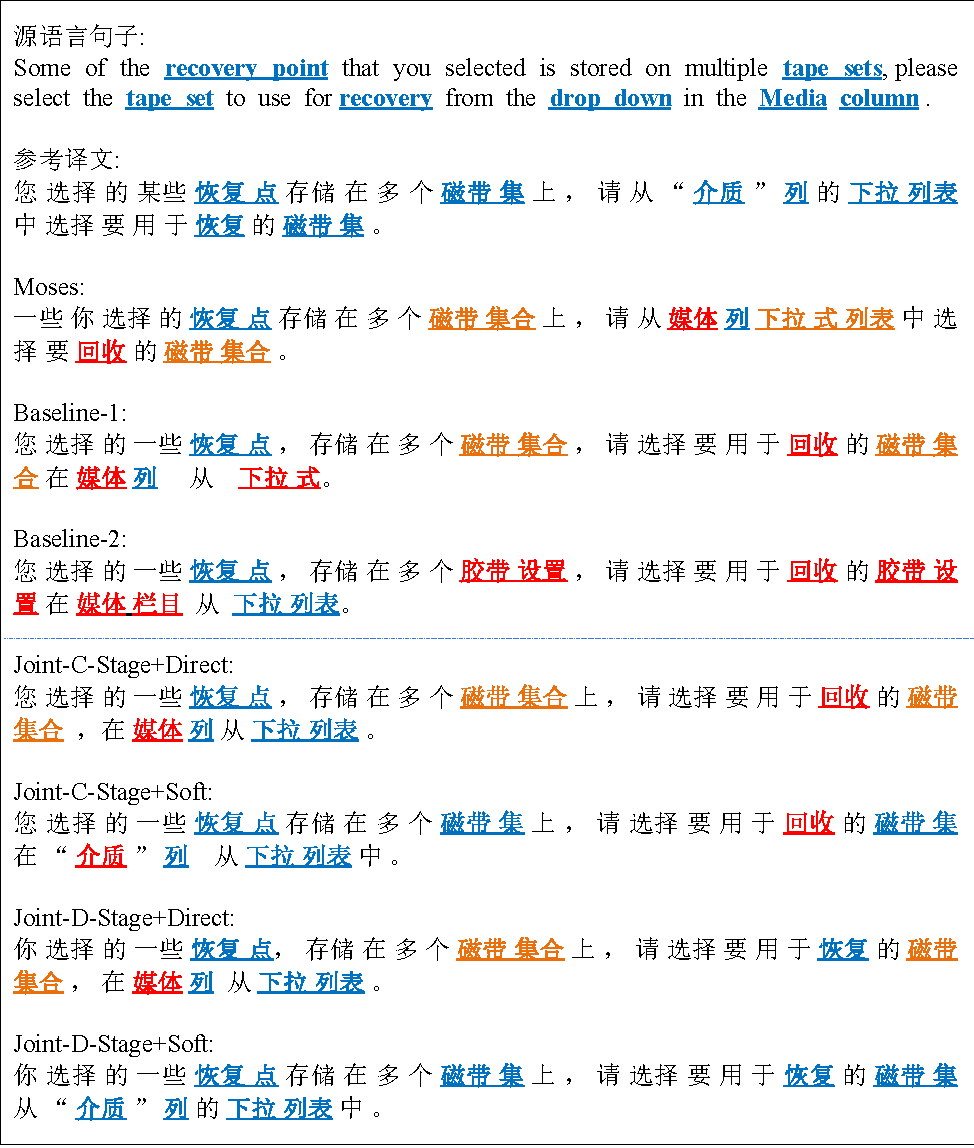
\includegraphics[width=0.95\textwidth]{Figure/Figure_4_7.pdf}
	\caption{四阶段联合模型术语直接翻译方法与柔性翻译方法的性能比较}
	\label{Fig_term_joint_example}
\end{figure}

在图\ref{Fig_term_joint_example}的上半部分,Moses的结果中,一共7个术语,我们可以发现有2个术语被完全正确翻译(蓝色),另外3个术语的译文虽然不完美但不影响阅读(橙色),剩下的2个术语完全被错误翻译而影响阅读和理解(红色)。在人机交互翻译过程中,橙色和红色所示的术语翻译都需要经过译员仔细的修改才可被接爱。

相对而言,我们实现的基线系统“Baseline-1”给出的译文的质量比较差,有3个术语被错误翻译,且译文的连贯性也相对较差。基线系统“Baseline-2”以流水线方法引入术语翻译之后的译文质量为最差,7个术语中有四个被错误翻译,译文连贯性也没有改善。这符合我们的实验预期。最直接的原因就是在术语识别分类器的性能比较低的情况下,直接从大规模双语术语词典中进行独立于上下文的查找和匹配,获得的译文质量很难比不考虑术语翻译的方法好。

根据图\ref{Fig_term_joint_example}的下半部分,我们提出的联合模型明显改善了术语和句子的翻译质量。我们可以看到,使用术语识别与双语术语对齐联合执行后,虽然直接翻译术语的译文质量(“Joint-C-Stage+Direct”)稍弱于Moses输出的译文,但相对于我们自己实现的基线系统“Baseline-1”和“Baseline-2”的原有结果仍有显著提升。值得注意的是,相同条件下,换用融合术语识别边界信息的统计翻译术语解码方法之后的译文质量(“Joint-C-Stage+Soft”)有明显改善:7个术语中的5个被完全正确翻译,与Moses的结果相比,可读性已经有明显改善。再通过对比“Joint-D-Stage+Direct”与“Joint-D-Stage+Soft”的译文质量,我们发现后者的术语已被完全正确翻译,且整句翻译质量明显优于Moses的译文质量。因此,我们可以作如下结论:与术语直接翻译的方法相比,在同等条件下,融合术语识别边界信息的统计翻译术语解码方法总能取得更好的翻译性能。

另外,通过对比“Joint-C-Stage+Direct”与“Joint-D-Stage+Direct”的译文质量,我们可以发现,让词对齐与单语术语识别和双语术语对齐融合后得到的翻译系统能翻译正确更多的术语,整句翻译质量也有明显改善。对比“Joint-C-Stage+Soft”与“Joint-D-Stage+Soft”,也可以得到相同的结论。因此,我们可以认为提出的四阶段联合模型确实有助于提高人机交互式机器翻译系统的可用性。
同理,通过对比“Joint-C-Stage+Direct”与“Joint-D-Stage+Soft”的译文质量,我们可以认为,在四阶段联合模型的基础上应用基于术语识别边界信息的统计翻译术语解码方法可以取得更好的翻译效果。

\section{本章小结}

在本章中,我们提出了基于术语识别边界信息的术语识别和翻译方法。由于当前术语识别的性能还比较低,该方法的基本思想是基于术语识别边界信息建立滑动窗口以动态扩展或收缩术语,借助术语识别边界信息建立术语解码方法,充分利用从平行句对和互联网单语语料中挖掘得到的术语翻译知识,包括三个部分:从平行句对中挖掘术语翻译知识的融合双语术语识别的联合词对齐模型,从单语语料中挖掘术语翻译知识的基于双语括号句子的术语挖掘方法,以及基于术语识别边界信息的统计翻译术语解码方法。实验结果表明,我们提出的基于术语识别边界信息的术语识别和翻译方法能显著提升计算机领域专业术语的翻译准确率,从而有效地改善了统计翻译译文质量。